\documentclass[a4paper,12pt]{article}
\usepackage{amsmath}
\usepackage{graphicx}
\usepackage[utf8]{inputenc}
\usepackage[english]{babel}
\usepackage[document]{ragged2e}
 
\begin{document}
\begin{flushleft}\newline \textbf{6.869 PSET 1}
\newline \textbf{09/14/2017}
\end{flushleft}
\newline \begin{center}\textbf{ISAAC KONTOMAH}
\end{center}
\newline \textbf{1.} \emph{\textbf{A simple Image Formation Model}}

\newline \emph{Orthographic Image:}The image shows three views , and can be viewed from the top(plan) and sides(side elevations) in 3d and it is not necessarily diminishing as you move further away from the camera.
\newline \emph{Perspective Image:} The image seems bigger and more prominent when nearer to the camera and diminishes when farther away.
\newline \textbf{2.} \emph{\textbf{Orthographic Projection}}
\newline Resultant =  Resolution in vertical axis + Resolution in horizontal axis
\newline $x=$ $Xcos(\theta)+ Xsin(\theta)$
\newline $x=$ $Xcos(0)+ Xsin(0)$
\newline $x=$ $X(1)+ X(0)$
\newline $= X$
\newline $y=$  $Ycos(\theta)-Zcos(90-\theta)$
\newline $y=$ $Ycos(\theta) -Z[cos(90)cos(\theta)+sin(90)sin(\theta)]$
\newline $y=$ $Ycos(\theta) -Z[0.cos(\theta)+1.sin(\theta)]$
\newline $y=$ $Ycos(\theta) -Z(sin(\theta))$
\newline $=Ycos(\theta) -Zsin(\theta)$
\newline \textbf{3.} \emph{\textbf{Constraints}}
\newline $Z(x,y)=0$ if $(x,y)$ belongs to a ground pixel
\newline $\frac{\partial Z}{\partial x}=$ undefined
\newline $Zsin(\theta)=Ycos(\theta)+y +y_{0}$
\newline $Z=Ycot(\theta)+\frac{y}{sin(\theta)}+\frac{y_{0}}{sin(\theta)}$
\newline $\frac{\partial Z }{\partial y}=\frac{1}{sin(\theta)}(1-\frac{\partial Y}{\partial y}cos(\theta)
)=\frac{1}{sin(\theta)}[1-\frac{1}{cos(\theta)}cos(\theta)
]=0$
\newline $\frac{\partial Z }{\partial t}= 0$
\newline $\frac{\partial^{2}Z}{\partial x^{2}}=0$
\newline $\frac{\partial^{2}Z}{\partial y^{2}}=\frac{\partial}{\partial y}(\frac{\partial Z}{\partial y})$
\newline $=\frac{\partial}{\partial y}(0)=0$
\newline $\frac{\partial^{2}Z}{\partial x \partial y}=\frac{\partial}{\partial x}(\frac{\partial Z}{\partial y})$
\newline $=\frac{\partial}{\partial x}[\frac{1}{sin(\theta)}]=0$
\newline \textbf{4.} \emph{\textbf{Approximation of derivatives}}
\newline \emph{\textbf{Line 166}}
\newline $\frac{\partial Y}{\partial t}=\frac{-n_{y}}{8}\frac{\partial Y}{\partial x}+ \frac{n_{x}}{8}\frac{\partial Y}{\partial y}$
\newline \[=
  \frac{-n_{y}}{8}\left( {\begin{array}{ccc}
   -1 & 0 & 1\\
   -2 & 0 & 2 \\
   -1 & 0 & 1 \\
  \end{array} } \right)   + \frac{n_{x}}{8}\left( {\begin{array}{ccc}
   -1 & -2 & -1\\
   0 & 0 & 0 \\
   1 & 2 & 1 \\
  \end{array} } \right) 
  \]
  \newline $=\frac{1}{8}\left[ {\begin{array}{ccc}
   n_{y}-n_{x} & -2n_{x} & -(n_{x}+n_{y)\\
   2n_{y} & 0 & -2n_{y} \\
   n_{x}+n_{y} & 2n_{x} & n_{x}-n_{y \\
  \end{array} } \right] $
  \newline \emph{\textbf{Line 180}}
  \newline After increment , kernel 
  $= A_{i,j}^{T}=0.1\left[ {\begin{array}{ccc}
   0 & -1& 0\\
   0 & 2 & 0 \\
   0 & -1 & 0 \\
  \end{array} } \right]^{T}= 0.1\left[ {\begin{array}{ccc}
   0 & 0& 0\\
   -1 & 2 & -1 \\
   0 & 0 & 0 \\
  \end{array} } \right] $

\newline \textbf{5.} \emph{\textbf{Run the Code}}

\newline Image Viewpoints

\begin{figure}
  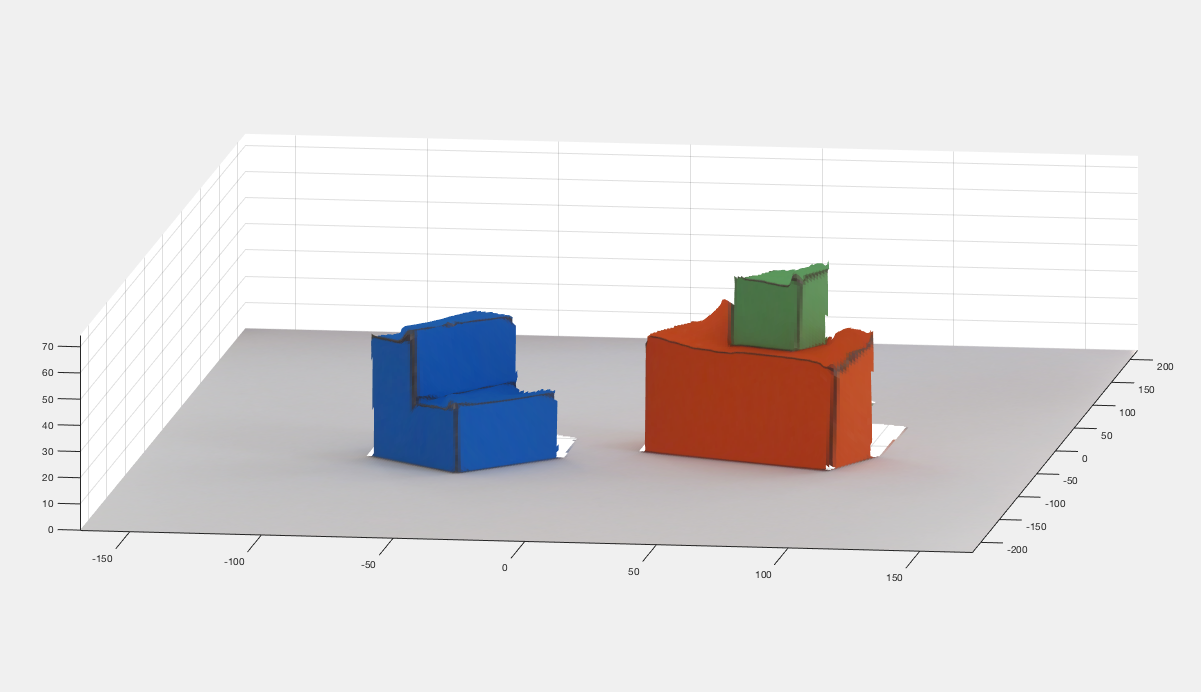
\includegraphics[width=\linewidth]{img2fig3.jpg}
  \caption{Image viewpoint , problem 5}
  \label{fig:Image viewpoint 1}
\end{figure}
\begin{figure}
  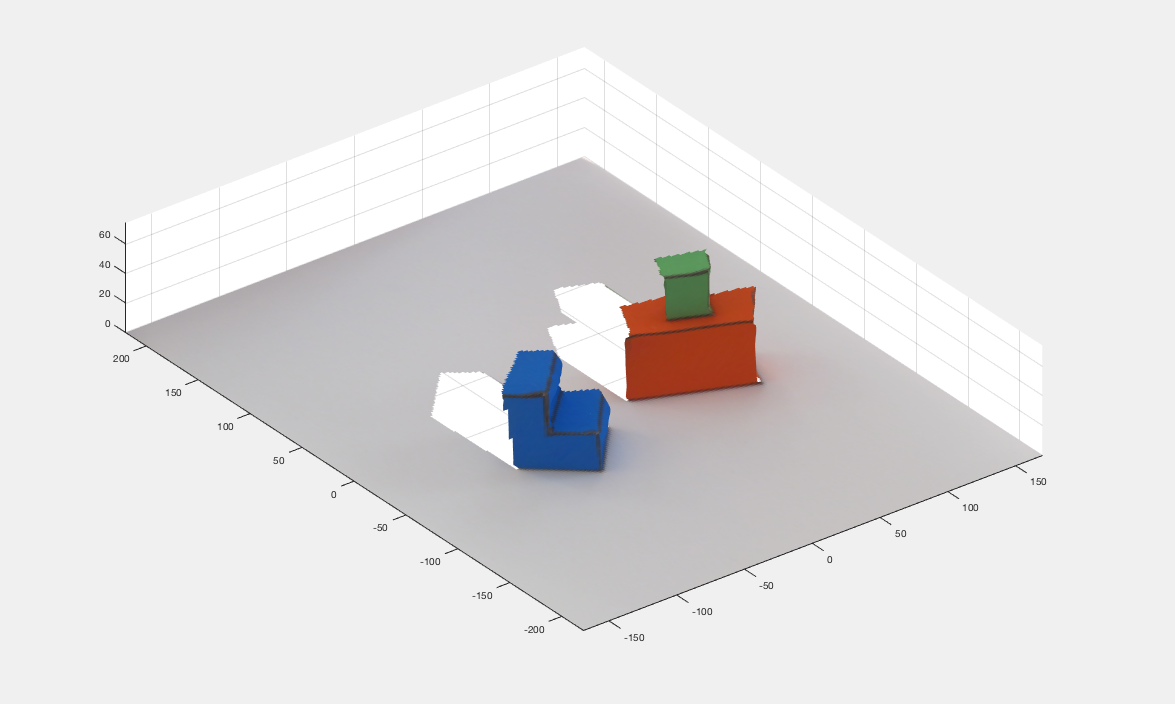
\includegraphics[width=\linewidth]{img2fig.jpg}
  \caption{Image viewpoint, problem 5}
  \label{fig:Image viewpoint 1}
\end{figure}
\begin{figure}
  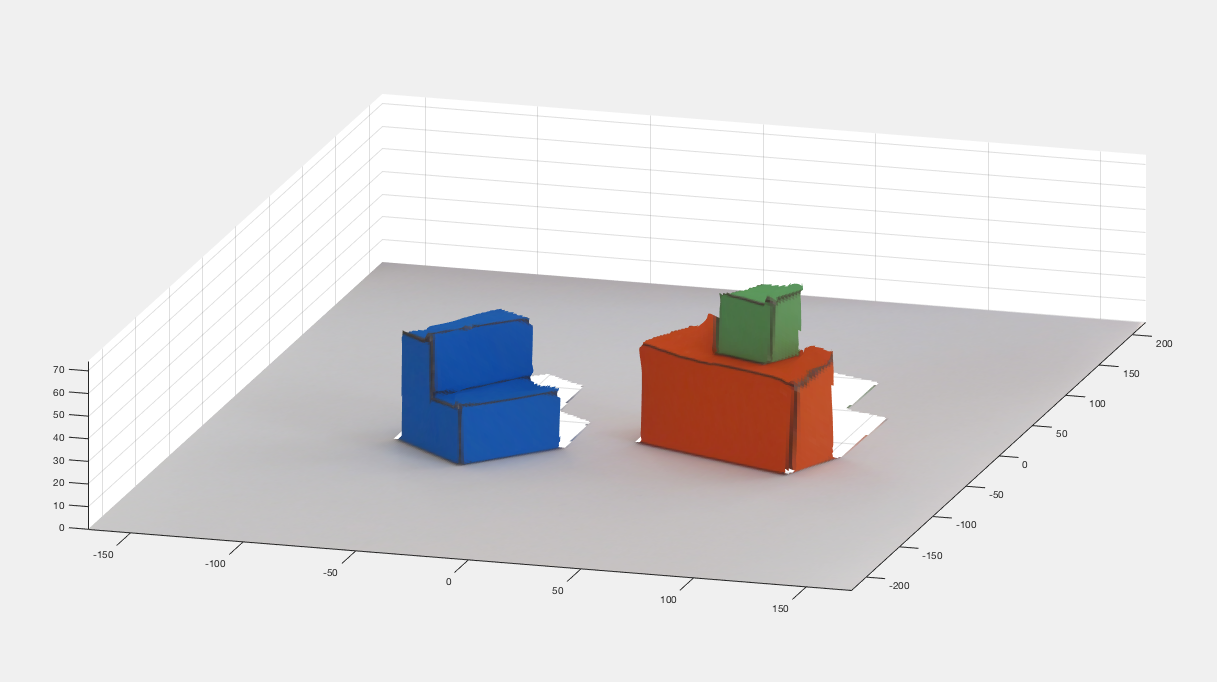
\includegraphics[width=\linewidth]{img2fig2.jpg}
  \caption{Image viewpoint,problem 5}
  \label{fig:Image viewpoint 1}
\end{figure}
\newline \begin{figure}
  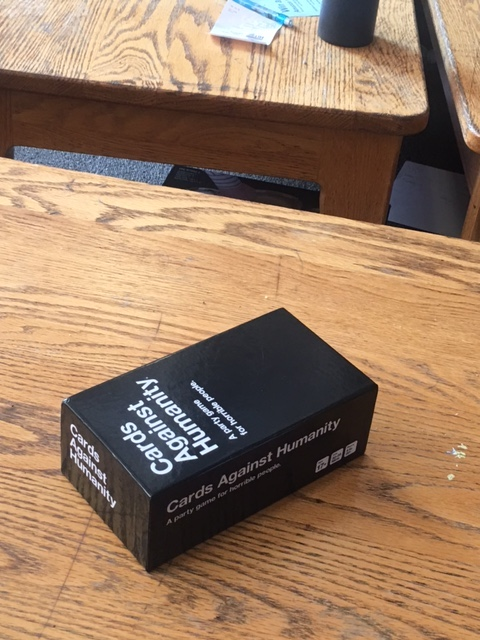
\includegraphics[width=\linewidth]{orthographic.jpg}
  \caption{Orthographic Image , problem 1.}
  \label{fig:orthographic image}
\end{figure}
\begin{figure}
  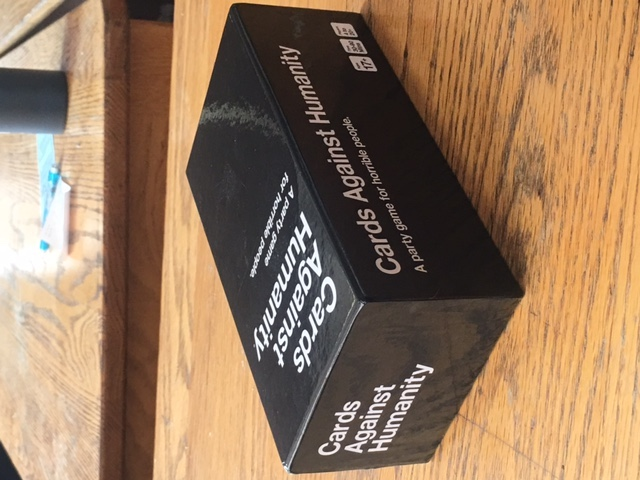
\includegraphics[width=\linewidth ,angle =270 ]{perspective.jpg}
  \caption{perspective Image , problem 1}
  \label{fig:perspective image}
\end{figure}
\begin{figure}
  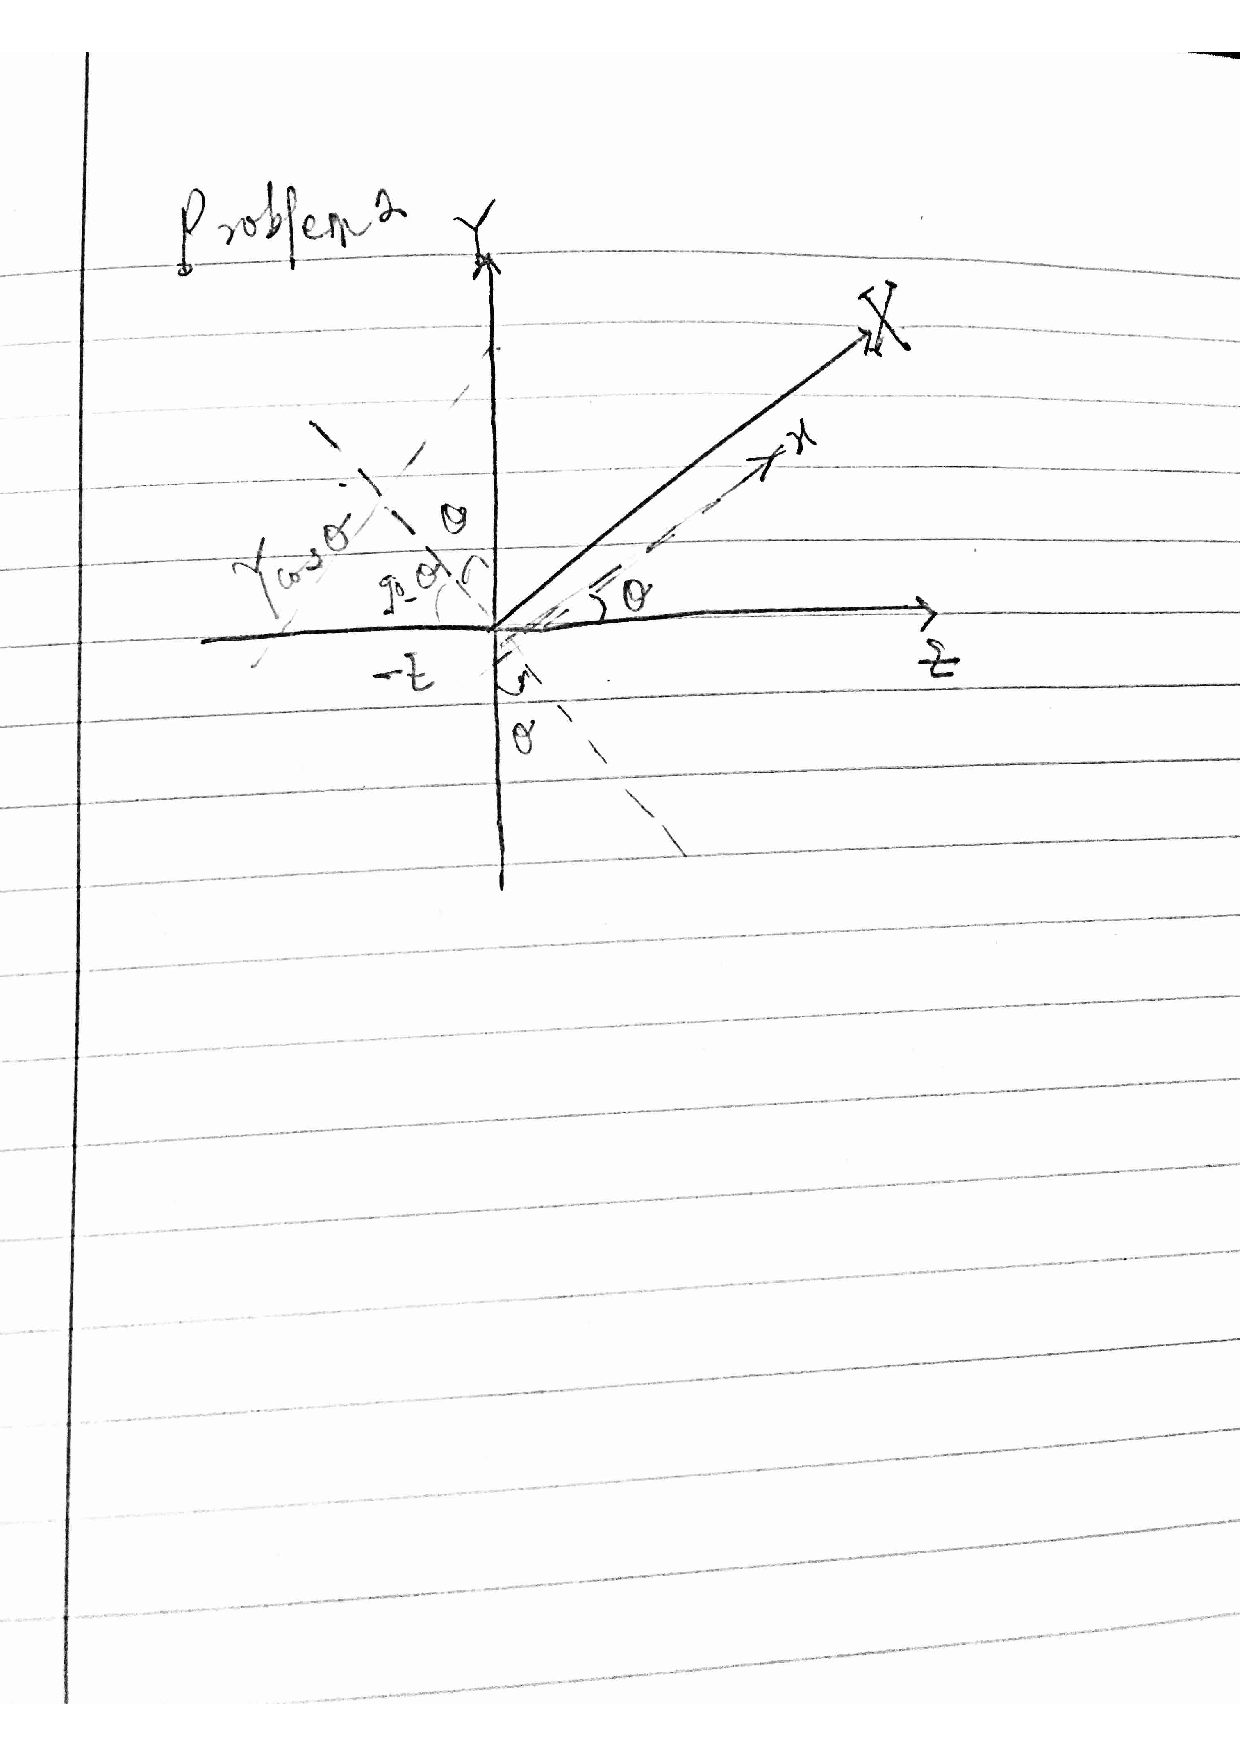
\includegraphics[width=\linewidth]{prob2.pdf}
  \caption{Resolution of vectors , problem 2 }
  \label{fig:Resolution of vectors}
\end{figure}
\newline \textbf{6.} \emph{\textbf{Violating simple world assumptions}}
\newline Image 3 fails
\newline Reason : You might miss an edge due to space not being enough between the red cube and the blue L shaped object , edge and the ground ,so not enough contrast, hence when taking a gradient you smooth over or ignore some edges and miss them
\end{document}